\section{Related Work}

\begin{frame}
\frametitle{Related Work}
\framesubtitle{Driver Monitoring Datasets}

\begin{itemize}
    \item AUC-DD \cite{abouelnaga2018real} is the first public dataset for DMSs. It was collected using an RGB camera from a single side view and thus have some limitations.
\end{itemize}

\begin{figure}
    \centering
    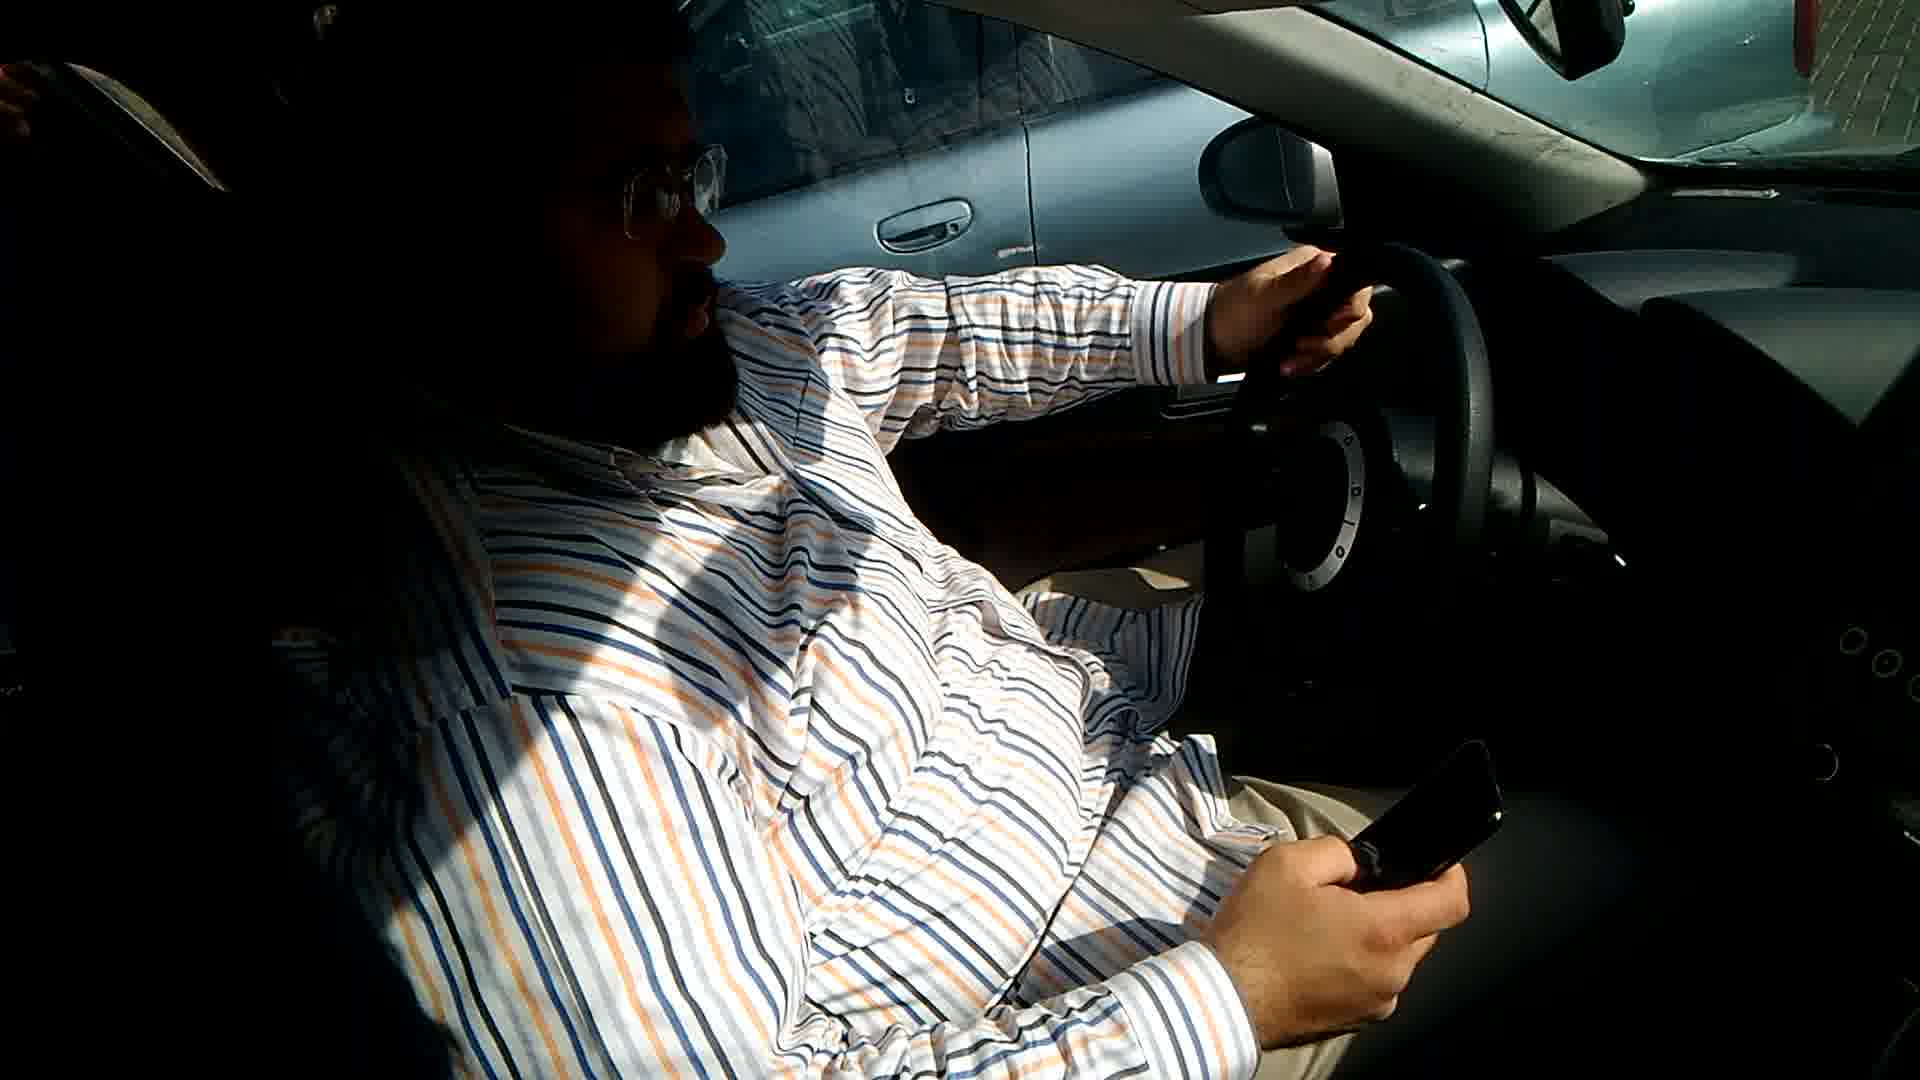
\includegraphics[width=0.5\textwidth]{images/auc-dd.jpg}
    \caption{A sample from the AUC-DD dataset \cite{abouelnaga2018real} illustrating that RGB is not robust to illumination changes.}
    \label{fig:3}
\end{figure}

\end{frame}

\begin{frame}
\frametitle{Related Work}
\framesubtitle{Driver Monitoring Datasets}

\begin{itemize}
    \item Later databases \cite{martin2019drive, ortega2020dmd, jegham2020novel, kopuklu2021driver} have incorporated additional views and modalities to address these issues.
        \begin{itemize}
            \item For example, top and front views have also been introduced to capture the driver's hand and head movements amongst other movements. 
            \item Regarding modalities, IR and depth have also become popular, as they can provide thermally based features and geometry information, which are complementary to the optical details from RGB.
        \end{itemize}
    \item Among these datasets, we benchmark our models on DAD \cite{kopuklu2021driver}, the only one designed for SAE L2+ with open-set recognition: its test set contains extra classes of NDRAs in addition to those in the training split.
\end{itemize}

\end{frame}

\begin{frame}
\frametitle{Related Work}
\framesubtitle{Multimodal DMSs}

Various multiview multimodal DMSs have also been proposed with different emphases:
\begin{itemize}
    \item Kopuklu \textit{et al.} \cite{kopuklu2021driver} proposed a novel learning framework based on contrastive learning.
    \item Ortega \textit{et al.} \cite{ortega2020dmd} and Su \textit{et al.} \cite{su2022efficient} proposed to leverage Conv-LSTM structures.
    \item Only Shan \textit{et al} \cite{shan2022multi} proposed a feature-level modality fusion method, but it has several drawback:
    \begin{itemize}
        \item Features are pooled before fusion, which leads to the loss of semantic information.
        \item Its fusion module has the additional task of handling the temporal dimension.
    \end{itemize}
\end{itemize}

\end{frame}